\documentclass[11pt,a4paper]{article}
\usepackage[margin=2.6cm]{geometry}
\usepackage{amsmath,amssymb}
\usepackage{booktabs,array}
\usepackage{enumitem}
\usepackage{xcolor}
\usepackage{graphicx}
\graphicspath{{figs/}}
\usepackage{tikz}
\usepackage[colorlinks=true,linkcolor=teal!70!black,citecolor=teal!70!black,urlcolor=teal!70!black]{hyperref}

\definecolor{bandA}{HTML}{008A7C}
\definecolor{bandB}{HTML}{C2610C}

% Full paper v2 (session 13, 2026-10-28): 3+1 storyline rewritten around the likelihood fit (Johnston reproduced -> where his error lives -> do not invert
% small counts -> Poisson likelihood of related-pair counts (Casasola's) from an intrinsic start -> checks, second shape, cost). Switch, weighted map, binomial term,
% eigenmaps, Madsen charts moved to App. A. Sections 1-7 unchanged from v1 (archive/counting-full-v1.tex). r25 (slab at equal density) filled in session 14.
% Session 14: r25 filled, author line, code URL (github.com/presindev/causet-counting), AI statement approved; endorser not needed (Roberto has gr-qc papers).

\title{Geometry by counting in causal sets:\\ exact $1+1$ tools, and spatial distances in $3+1$}
\author{Roberto Bada\\ \small SapereIA, Barcelona, Spain\\ \small Institute of Cosmos Sciences, University of Barcelona (ICCUB), Barcelona, Spain\\ \small \texttt{roberto@sapereia.com}}
\date{Draft v2, 28 October 2026}

\emergencystretch=1.5em
\begin{document}
\maketitle

\begin{abstract}
In causal set theory spacetime is a locally finite partial order, and geometry must be read from the order and from counting. We collect and test counting tools, exact in $1+1$ dimensions and approximate in $3+1$. (i) For two spacelike events, the volumes of the causal-overlap regions of Bogu\~n\'a and Krioukov with respect to \emph{any} event $c$ in their common past obey an exact identity in flat $1+1$ spacetime, $d^2=2V_AV_B/V_C$; with a Poisson bias correction the estimate is unbiased above two discreteness lengths. (ii) In curved spacetime the estimate drifts with the depth of $c$; in de Sitter space the drift is exactly $\tanh^2(H\tau/2)/[2\ln\cosh(H\tau/2)]=1-R\tau^2/16+\dots$, which gives a curvature estimator. (iii) We calibrate the Lorentzian-embedding test of Clough and Evans against size and curvature, show that it misses layered orders, and add the share of zero-length pairs as the missing flag; the combined test separates the two phases of $e^{-\beta S}$ models at $N=200$ and $400$, including on held-out chains. (iv) For Johnston's chain-sum propagator the mean over intervals of exactly $n$ elements in a random 2D order is $\tfrac12L_n(m^2/2\rho)$, a density-free target. (v) In $3+1$ dimensions we reproduce Johnston's 2025 embedding and locate its error: it comes entirely from spacelike pairs, and almost entirely from pairs whose shared regions hold fewer than ten events. Turning such small counts into distances cannot fix this at any size, as a counting argument shows, even with an exact (tabulated) inversion of the Bogu\~n\'a--Krioukov overlap for any reference event. Fitting the spatial coordinates directly to the interval counts of all related pairs, with their Poisson noise (Casasola's likelihood), started from a map built from counts, removes $79$--$83\%$ of Johnston's residual error at every size from $n=3000$ to $15000$ events, in all 21 universes; the fit is consistent and independent of the start. A term of our own for the spacelike overlap counts makes it worse. In a second shape without a waist, at equal density, the gain is $58$--$65\%$ ($80$--$86\%$ on interior pairs); the loss against the diamond comes entirely from intervals cut by the side wall. The work was done in under a week by one physicist working with an AI system; we describe how, and how the results were checked (Sec.~\ref{sec:method}).
\end{abstract}

\section{Introduction}
A causal set is a set of events with a partial order (``$x$ precedes $y$'') that is locally finite: every interval $I(x,y)=\{z:x\prec z\prec y\}$ is finite~\cite{BLMS87,Surya19}. The hypothesis of causal set theory is that spacetime is such a set, with the continuum a large-scale approximation. Order and number then carry all the geometry: the number of events in a region measures its volume, and the order fixes the light cones. The kinematic programme is to recover everything else from these two.

Some of this is classical. The longest chain between two events estimates their proper time~\cite{BrightwellGregory91}; interval and chain abundances give the dimension and curvature~\cite{RSS13,GlaserSurya13}; the Benincasa--Dowker operator gives the scalar curvature and the action~\cite{BD10,DowkerGlaser13}. Spatial distance is harder, because spacelike events have no interval between them. Bogu\~n\'a and Krioukov recently measured it through the overlap of the pasts of two events, seen from an event $c$ at equal proper time below both~\cite{BK24}; Hu, Meyer and Meyer gave an exact $1+1$ reconstruction from a past and a future event~\cite{HMM25}. Whether a given causal set looks like a manifold at all is tested by dimension estimators, interval abundances~\cite{GlaserSurya13} and Lorentzian embeddings~\cite{CloughEvans16,Henson06,Johnston25}. On the dynamical side, matter can be put on the order through Johnston's sum over chains~\cite{Johnston08,Johnston09}, whose average over sprinklings reproduces the Klein--Gordon propagator.

This paper adds four small, checkable pieces in $1+1$ dimensions and one comparison in $3+1$, and tests each on Poisson sprinklings against the known continuum:
\begin{enumerate}[leftmargin=*,itemsep=1pt]
\item a rectangle identity that frees the overlap distance from the equal-time choice of $c$ (Sec.~\ref{sec:dist});
\item curvature from the way that estimate drifts with the depth of $c$, with a closed form in de Sitter space (Sec.~\ref{sec:curv});
\item a calibration of the Lorentzian-embedding test against size and curvature, and a blind spot for layered orders with its fix (Sec.~\ref{sec:embed}), applied to classical growth and to the two phases of $e^{-\beta S}$ models (Sec.~\ref{sec:phases});
\item an exact, density-free target for Johnston's propagator at fixed interval size (Sec.~\ref{sec:prop});
\item in $3+1$ dimensions, a head-to-head test against Johnston's recent embedding~\cite{Johnston25}: where his error lives, why distances inverted from small counts cannot fix it, and a likelihood fit to the counts, from an intrinsic start, that removes about $80\%$ of it (Sec.~\ref{sec:3p1}).
\end{enumerate}
The $1+1$ pieces are elementary; we think they are useful, and we did not find them in the literature. The $3+1$ result is a large improvement on the current state of the art for spatial distances, obtained with a likelihood that already exists~\cite{Casasola26} and that we credit; ours are the diagnosis, the intrinsic start and the test. Sec.~\ref{sec:disc} lists what we checked; App.~\ref{app:dropped} lists what we tried and dropped. All code is available (see the end).

The paper is also a report on a way of working. Everything in it was produced in six days (24--29 October 2026) by one physicist, new to causal sets, working with an AI system as a research partner. Sec.~\ref{sec:method} describes the division of labour, the checks that replaced the slower human ones, and the mistakes that the process caught; we think the method is as much a result as the physics, and we report it so that it can be judged and reused.

\section{How this work was done}\label{sec:method}
% Roberto's choices (session 12): main-text section, given prominence; roles, checks, mistake log, public notebook; he checked derivations and the final text and set
% the direction, but did not check the code line by line; name the model and tool; SapereIA affiliation + funding; ICCUB/LVK background.
\paragraph{Who did it.} The author is a physicist who works in gravitational-wave research with the Institute of Cosmos Sciences of the University of Barcelona (ICCUB) and is a member of the LIGO--Virgo--KAGRA Collaboration; this paper is not a product of that collaboration and lies outside its scope. As a co-founder of SapereIA he studies how AI systems can help to advance scientific knowledge, and this project was set up partly as a test of that question: could one physicist, new to a field, and an AI system working as a colleague reach results that are new, checked and publishable, in days rather than months? The AI system was Claude Opus~5.5 (Anthropic), used through the Claude Code command-line tool, which can read and write files, run code locally and submit jobs to a computing cluster. It is not an author.

\paragraph{What happened, and how fast.} The work ran over fourteen sessions of a few hours each, between 24 and 29 October 2026, as a conversation recorded in a research notebook (idea files, a journal per session, a log of mistakes, a record of dead ends). Table~\ref{tab:timeline} lists when each result of this paper appeared. Along the way the project produced about 6000 lines of simulation code in 63 scripts, about 30 cluster jobs, and six internal drafts, each with a written review against the standard of an arXiv preprint.

\begin{table}[h]
\centering\small
\begin{tabular}{@{}lll@{}}
\toprule
Day & Sessions & Results that entered this paper \\
\midrule
24 Oct & 1 & starting idea: discrete spacetime from counting \\
25 Oct & 2--6 & rectangle identity, depth drift (Secs.~\ref{sec:dist},~\ref{sec:curv}); first embedding test; first cluster runs \\
26 Oct & 7 & fixed-$n$ propagator target (Sec.~\ref{sec:prop}) \\
27 Oct & 8--11 & phases at $N=400$; literature crawl (credit to~\cite{CloughEvans16}); detector fix; figures; \\
 & & $3+1$ estimator; reproduction of~\cite{Johnston25}; oracle; switch \\
28 Oct & 12--13 & large-$n$ cluster verdict; diagnosis of the low-count pairs; likelihood fit, \\
 & & ablation and literature search (credit to~\cite{Casasola26}); second shape; this draft \\
29 Oct & 14 & second shape at equal density (Sec.~\ref{sec:3p1}); final literature check; release \\
\bottomrule
\end{tabular}
\caption{When each result appeared. A session is one sitting of a few hours.}\label{tab:timeline}
\end{table}

\paragraph{Roles.} The author brought in the paper that started the distance work, Bogu\~n\'a and Krioukov's overlap method~\cite{BK24}, on which Secs.~\ref{sec:dist} and~\ref{sec:3p1} build; he proposed the questions and most of the ideas that ended up working (among them the switch of App.~\ref{app:dropped}, from his suggestion to use each method only where it is good, and the questions that led to the low-count diagnosis and the second shape), set the physical constraints the models had to respect, and decided which lines to pursue or drop. The AI system searched and read the literature, carried out the derivations, wrote and ran the simulation code (on a laptop and on the ICCUB cluster), and drafted the text. The author followed and checked the derivations, and read and approved the final text; he did not review the code line by line. The numerical claims therefore rest on the checks below rather than on independent human review of the code.

\paragraph{Checks.} Speed is only worth something if the results hold, so the working rules were built around catching errors. Every tool was first run on a case with a known answer (flat space, de Sitter, the continuum limit) before being applied to anything else. The published numbers of the method we compare against were reproduced before any comparison~\cite{Johnston25}. Any parameter chosen while looking at the data was re-tested on fresh random seeds, and every comparison is paired: the same universes for every method. Before calling something new, we read the full citation lists of the closest papers and searched the citing papers' full texts; Sec.~\ref{sec:disc} states what was checked for each claim. All quoted numbers were rerun from the scripts with fixed seeds.

\paragraph{Mistakes.} Errors were frequent, and most were the AI system's; what mattered was that they were caught and written down. The notebook's mistake log has 41 entries, each with the working rule it produced, and the dead ends are kept with the reason they died. Examples that changed this paper: a ``hysteresis'' that came from Monte Carlo chains with acceptance below $10^{-3}$, i.e.\ frozen (withdrawn); a detector we believed new that turned out to be Clough and Evans's~\cite{CloughEvans16} (now credited); a comparison with~\cite{Johnston25} that had put two different distances side by side (redone on the same quantity); a counts-only map that matched~\cite{Johnston25} up to $n=3000$ events but lost at larger $n$ (dropped); and a likelihood fit first presented as resting on a new term of ours, until removing each term in turn showed that the gain comes from the related-pair term, which is Casasola's~\cite{Casasola26}, while ours makes it worse (now credited, and our term dropped). The $3+1$ dead ends are listed in App.~\ref{app:dropped}.

\paragraph{What this does and does not show.} One project is an anecdote, not a measurement. The results are modest in size, they have not yet been refereed, and a reader who wants to verify them should run the code rather than trust the process. What the project does show is that, with an AI system doing the reading, the algebra and the programming, and with explicit rules against self-deception, a physicist from a neighbouring field can go from a first idea to a reproduction of a 2025 result, a diagnosis of its error and a large improvement on it in a few days, provided that the literature search is redone before every claim of novelty.

\paragraph{Availability.} The code and the full notebook (idea files, session journal, mistake log, dead ends, internal drafts and their reviews) are public at \url{https://github.com/presindev/causet-counting}, as a snapshot; only the notes on the computing cluster's internal configuration are left out.

\section{Setting}\label{sec:setting}
We generate test universes by sprinkling: a Poisson process of density $\rho$ in a region of a known spacetime, with the order induced by the light cones. We then discard the coordinates and compare what the counting tools find with the truth. In $1+1$ dimensions we write $\ell=\rho^{-1/2}$ for the discreteness length: a patch of volume $\ell^2$ holds one event on average; in $3+1$ dimensions $\ell=\rho^{-1/4}$.

We use light-cone coordinates $u=t-x$, $v=t+x$, in which $dt\,dx=du\,dv/2$ and $x\prec y$ iff $u_x<u_y$ and $v_x<v_y$. The interval between $x\prec y$ is the rectangle $[u_x,u_y]\times[v_x,v_y]$, with volume $V=\Delta u\,\Delta v/2=\tau^2/2$. A sprinkled causal diamond is therefore a uniformly random \emph{2D order}: the intersection of two random linear orders~\cite{BHS08,Surya12}. For two spacelike events $d^2=\Delta x^2-\Delta t^2=-\Delta u\,\Delta v$.

Errors quoted are standard errors over independent sprinklings unless stated otherwise. The proper time from the longest chain has mean $\simeq2\sqrt n$ in an interval of $n$ events, with Tracy--Widom fluctuations of size $\simeq n^{1/6}$~\cite{BDJ99}; we use the count instead, $\tau^2=2n/\rho$, wherever a volume is available.

\section{Distance: a rectangle identity}\label{sec:dist}
Let $a,b$ be spacelike and $c$ an event in their common past. Following~\cite{BK24}, split the two intervals into
\begin{equation}
A=I(c,a)\setminus I(c,b),\qquad B=I(c,b)\setminus I(c,a),\qquad C=I(c,a)\cap I(c,b).
\end{equation}
Bogu\~n\'a and Krioukov choose $c$ at equal proper time $\tau_c$ below $a$ and $b$ and derive $d$ from the overlap fraction. In $1+1$ dimensions the choice of $c$ does not matter, because of the following identity (Fig.~\ref{fig:tiles}).

\begin{figure}[t]
\centering
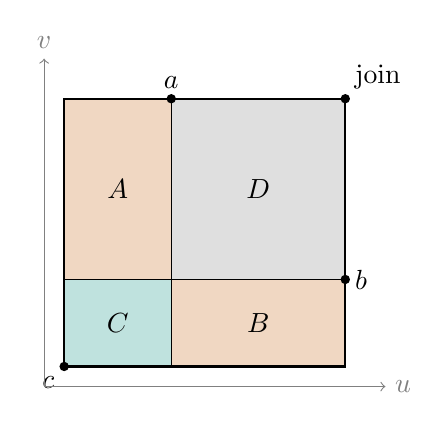
\begin{tikzpicture}[scale=0.85]
  \fill[bandA!25] (0,0) rectangle (1.6,1.3);
  \fill[bandB!25] (0,1.3) rectangle (1.6,4);
  \fill[bandB!25] (1.6,0) rectangle (4.2,1.3);
  \fill[gray!25] (1.6,1.3) rectangle (4.2,4);
  \draw[thick] (0,0) rectangle (4.2,4);
  \draw (1.6,0) -- (1.6,4); \draw (0,1.3) -- (4.2,1.3);
  \node at (0.8,0.65) {$C$}; \node at (0.8,2.65) {$A$}; \node at (2.9,0.65) {$B$}; \node at (2.9,2.65) {$D$};
  \fill (0,0) circle (2pt) node[below left] {$c$};
  \fill (1.6,4) circle (2pt) node[above] {$a$};
  \fill (4.2,1.3) circle (2pt) node[right] {$b$};
  \fill (4.2,4) circle (2pt) node[above right] {join};
  \draw[->,gray] (-0.3,-0.3) -- (4.8,-0.3) node[right] {$u$};
  \draw[->,gray] (-0.3,-0.3) -- (-0.3,4.6) node[above] {$v$};
\end{tikzpicture}
\caption{The rectangle identity in light-cone coordinates (rotate by $45^\circ$ for the usual picture). The rectangle from $c$ to the join of $a$ and $b$ splits into the overlap $C$, the strips $A$ and $B$ seen by only one of $a,b$, and the tile $D$ with $a$ and $b$ at opposite corners. Opposite tiles have equal products, $V_CV_D=V_AV_B$, and $V_D=d^2/2$.}
\label{fig:tiles}
\end{figure}

\paragraph{Derivation.} Put $c$ at the origin and take $u_a<u_b$, $v_a>v_b$ ($a$ and $b$ spacelike). Then $I(c,a)=[0,u_a]\times[0,v_a]$ and $I(c,b)=[0,u_b]\times[0,v_b]$. The rectangle from $c$ to the join $(u_b,v_a)$ splits into four tiles,
\begin{equation}
C=[0,u_a]\times[0,v_b],\quad A=[0,u_a]\times[v_b,v_a],\quad B=[u_a,u_b]\times[0,v_b],\quad D=[u_a,u_b]\times[v_b,v_a].
\end{equation}
With $\Delta u=u_b-u_a$ and $\Delta v=v_a-v_b$ the volumes are $V_C=u_av_b/2$, $V_A=u_a\Delta v/2$, $V_B=\Delta u\,v_b/2$, $V_D=\Delta u\,\Delta v/2$, so $V_CV_D=V_AV_B$. The tile $D$ has $a$ and $b$ at opposite corners, so $V_D=\Delta u\,\Delta v/2=d^2/2$. Hence, for every $c$ in the common past,
\begin{equation}
d^2=\frac{2V_AV_B}{V_C}.
\label{eq:rect}
\end{equation}
The tile $D$ is the interval between the meet and the join of $a$ and $b$, i.e.\ the $1+1$ ``naive'' spatial distance of Brightwell and Gregory and of Rideout and Wallden, who take the minimal interval between a common past and a common future event~\cite{BrightwellGregory91,RideoutWallden09}; what the identity adds is that this volume can be read from the past alone, through one event $c$. The equal-time choice of~\cite{BK24} is $V_A=V_B$, and their $1+1$ formula reduces to Eq.~\eqref{eq:rect} in that case; with a general $c$ the search for equal-time events, which needs the density and the dimension~\cite{BK24}, is not needed. The identity uses that the overlap of two $1+1$ intervals is again an interval; in more dimensions it is not, and Eq.~\eqref{eq:rect} has no direct analogue.

\paragraph{Estimator.} On a causal set, $V_X$ is replaced by $N_X/\rho$, the number of events in the region. The three regions are disjoint, so $N_A$, $N_B$, $N_C$ are independent Poisson variables with means $\lambda_X=\rho V_X$. Then $N_AN_B$ is unbiased for $\lambda_A\lambda_B$, but $1/N_C$ is biased (and undefined at $N_C=0$). Since $E[1/(N+1)]=(1-e^{-\lambda})/\lambda$ for a Poisson variable,
\begin{equation}
\widehat{d^2}=\frac{2N_AN_B}{\rho\,(N_C+1)}
\label{eq:est}
\end{equation}
is unbiased up to $e^{-\lambda_C}$. Without the $+1$ a flat control read $11\%$ high at shallow $c$. The relative variance is about $1/\lambda_A+1/\lambda_B+1/\lambda_C$, so the deepest available $c$ is best. The strips $A$ and $B$ are long and thin, and hold many events even when $d\sim\ell$; this is why overlap estimators work down to the discreteness scale.

\paragraph{Test.} Table~\ref{tab:dist} and Fig.~\ref{fig:distance} use flat sprinklings in a unit diamond, random spacelike pairs among the late events, and for each pair the deepest $c$ (largest $N_C$). There is no measurable bias above $2\ell$, and the error at large $d$ falls roughly as $N^{-1/2}$. Below $2\ell$ the error stays near $20\%$ for all $N$: that is the discreteness scale itself.

\begin{table}[t]
\centering\small
\begin{tabular}{@{}rccc@{}}
\toprule
$N$ & $d<2\ell$ & $2\ell$--$10\ell$ & $>10\ell$\\
\midrule
1000 & 23\% & 6.5\% & 5.2\%\\
2000 & 15\% & 5.0\% & 3.4\%\\
4000 & 19\% & 5.1\% & 2.5\%\\
\bottomrule
\end{tabular}
\caption{Median relative error of Eq.~\eqref{eq:est} with the deepest $c$, flat $1+1$ sprinklings, 300 pairs $\times$ 4 sprinklings per $N$.}
\label{tab:dist}
\end{table}

\begin{figure}[t]
\centering
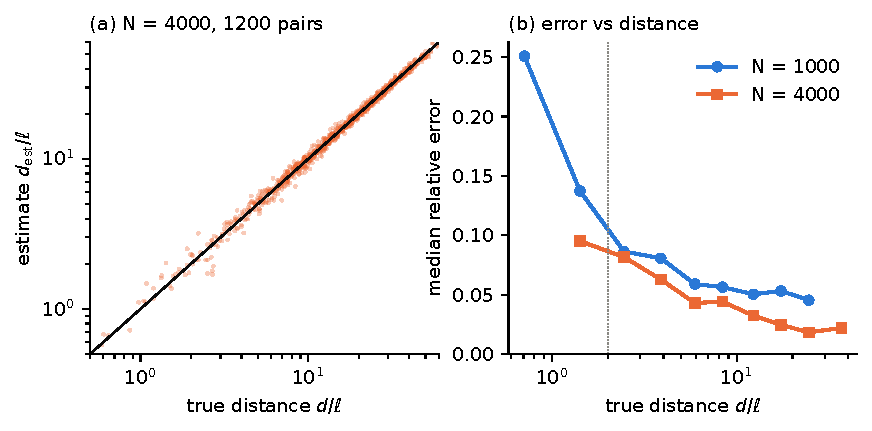
\includegraphics[width=0.92\linewidth]{fig_distance}
\caption{Eq.~\eqref{eq:est} with the deepest $c$ on flat $1+1$ sprinklings, from the causal order only. (a) Estimate against true distance, $N=4000$. (b) Median relative error per distance bin; the dotted line marks $2\ell$.}
\label{fig:distance}
\end{figure}

\section{Curvature from depth drift}\label{sec:curv}
In flat space every $c$ in the common past gives the same answer. In curved space Eq.~\eqref{eq:rect} is no longer exact, and the estimate depends on how deep $c$ lies. That dependence measures curvature.

\paragraph{de Sitter volumes.} Two-dimensional de Sitter space in conformal coordinates,
\[ds^2=\frac{-d\eta^2+dx^2}{(H\eta)^2},\qquad\eta<0,\]
has the same light cones as flat space. The tiles $A,B,C,D$ are the same rectangles in $(u,v)=(\eta-x,\eta+x)$, but volumes are weighted,
\[dV=\frac{d\eta\,dx}{(H\eta)^2}=\frac{2\,du\,dv}{H^2(u+v)^2}.\]
Integrating over $[u_1,u_2]\times[v_1,v_2]$, the inner integral gives $1/(u+v_1)-1/(u+v_2)$ and the outer one a logarithm:
\begin{equation}
V_\square=\frac{2}{H^2}\ln\frac{\eta_L\,\eta_R}{\eta_{\rm bot}\,\eta_{\rm top}},
\label{eq:dsvol}
\end{equation}
with $\eta=(u+v)/2$ evaluated at the left, right, bottom and top corners.

\paragraph{Closed form.} Put $a,b$ on one slice, $(\eta_0,\mp h)$, and $c$ straight below at $(\eta_0-T,0)$; set $H=1$. By symmetry $V_A=V_B$. From Eq.~\eqref{eq:dsvol}, to first order in $h$,
\begin{equation}
\begin{aligned}
V_A&=2\Big[\ln\big(q+\tfrac h2\big)+\ln(\eta_0-h)-\ln\big(q-\tfrac h2\big)-\ln\eta_0\Big]\\
&\simeq2h\Big(\frac1q-\frac1{\eta_0}\Big)=\frac{hT}{\eta_0\,q},\qquad q=\eta_0-\tfrac T2,
\end{aligned}
\end{equation}
and at $h=0$
\begin{equation}
V_C=2\ln\frac{q^2}{(\eta_0-T)\,\eta_0}=-2\ln(1-x),\qquad x=\frac{T^2}{4q^2}.
\end{equation}
The true distance is $d\simeq2h/|\eta_0|$. So
\begin{equation}
\frac{d^2_{\rm est}}{d^2}=\frac{2V_A^2/V_C}{4h^2/\eta_0^2}=\frac{x}{-\ln(1-x)}.
\end{equation}
The proper time from $c$ up to the midpoint of $a,b$ is $\tau=\ln(|\eta_0-T|/|\eta_0|)$, so $T/|\eta_0|=e^{\tau}-1$ and $x=\big((e^\tau-1)/(e^\tau+1)\big)^2=\tanh^2(\tau/2)$. Restoring $H$,
\begin{equation}
\frac{d^2_{\rm est}}{d^2}=\frac{\tanh^2(H\tau/2)}{2\ln\cosh(H\tau/2)}=1-\frac{(H\tau)^2}{8}+O(\tau^4)=1-\frac{R\,\tau^2}{16}+\dots,\qquad R=2H^2,
\label{eq:drift}
\end{equation}
exact as $d\to0$ at any depth (the denominator is $H^2/2$ times the de Sitter volume of an interval of height $\tau$, $V=(4/H^2)\ln\cosh(H\tau/2)$), and independent of $\eta_0$ as it must be by the symmetry of de Sitter space. We checked Eq.~\eqref{eq:drift} against the exact volumes, Eq.~\eqref{eq:dsvol}, to $10^{-5}$ for $H\tau=0.1$--$3$. A sideways offset of $c$ changes it little, and a finite $d$ adds a roughly depth-independent shift. Every $1+1$ metric is conformally flat, so the leading term should hold locally in any $1+1$ spacetime. We checked this beyond de Sitter in $1+1$ FRW spacetimes $ds^2=a(\eta)^2(-d\eta^2+dx^2)$ with $a=\eta^p$, where $R=2(\ln a)''/a^2=-2p\,\eta^{-2-2p}$ varies in time and the rectangle volumes have a closed form. For $p=1$, $-2$ and $\tfrac12$ (negative, positive and negative curvature), $16(1-d^2_{\rm est}/d^2)/\tau^2$ tends to $R$ at the location of $a,b$ as $\tau\to0$ (to $1\%$ at $\tau=0.01$), with the right sign: for $R<0$ the ratio rises above $1$. At finite depth it reads a curvature between the one at $a,b$ and the one at the proper-time midpoint: the drift averages $R$ over the region, weighted towards the top.

\paragraph{Test on sprinklings.} We sprinkle de Sitter ($H=1$, $\rho=10^4$) and, as a control, flat space in the same coordinates, insert $a,b$ by hand $\approx14\ell$ apart, and evaluate Eq.~\eqref{eq:est} for every sprinkled $c$ in their common past whose rectangle lies inside the region. Figure~\ref{fig:drift} shows the mean ratio per depth bin over 400 sprinklings against the continuum computed for the same $c$'s. The flat control stays at $1$ and de Sitter follows the continuum. Two cautions: neighbouring depth bins share events and are $\approx0.9$ correlated, so a run of deviations in adjacent bins is one fluctuation, not several (we saw a 2$\sigma$ run in a first batch of 100 sprinklings that disappeared in the next 300); and in the shallowest bin the tiles hold few events and the estimator reads low in both geometries.

\begin{figure}[t]
\centering
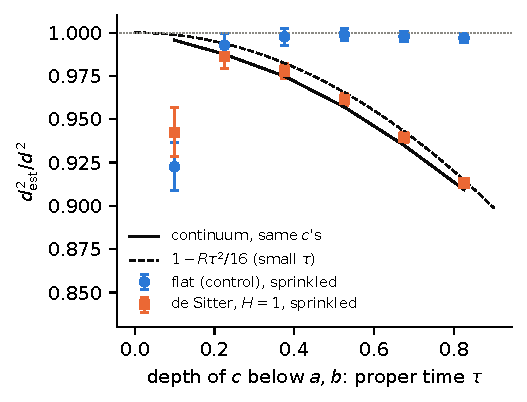
\includegraphics[width=0.52\linewidth]{fig_drift}
\caption{Depth drift of the rectangle estimate. Mean over 400 sprinklings ($\rho=10^4$) per bin of the proper time $\tau$ from $c$ up to $a,b$; errors from the spread between sprinklings. Solid: continuum ratio from the exact volumes, averaged over the same $c$'s. Dashed: the small-$\tau$ term of Eq.~\eqref{eq:drift}.}
\label{fig:drift}
\end{figure}

\paragraph{A curvature estimator.} Using only counts, fit $\widehat{d^2}=\alpha+\beta\tau^2$ over the $c$'s of one pair with $\tau\in[0.2,0.7]$ and $\tau^2=(N_{I(c,a)}+N_{I(c,b)})/\rho$, and set $R_{\rm est}=-16\beta/\alpha$. Over 100 sprinklings, one pair each:
\begin{center}\small
\begin{tabular}{@{}rccc@{}}
\toprule
$\rho$ & flat (true $R=0$) & de Sitter (true $R=2$; continuum fit $1.9$--$2.2$) & spread per pair\\
\midrule
4000 & $-0.7\pm0.6$ & $1.3\pm0.7$ & $\approx6$--$7$\\
$10^4$ & $0.3\pm0.4$ & $1.6\pm0.4$ & $\approx4$\\
\bottomrule
\end{tabular}
\end{center}
The continuum value depends on whether $\tau$ is the true proper time ($1.88$) or read from interval volumes as the counts do ($2.2$). In the $p=1$ FRW spacetime above ($\rho=10^4$, 200 sprinklings, $a,b$ at $\eta_0=1.5$), the binned ratio follows the exact continuum within $1\sigma$ for $\tau\ge0.15$, and the fit gives $R_{\rm est}=-1.25\pm0.30$ against $-0.81$ for the same fit on the continuum, while $R$ itself runs from $-0.4$ at $a,b$ to $-2.8$ at the bottom of the window. The fit therefore measures a depth-weighted average of $R$, not $R$ at $a,b$. The estimator is right on average and tells flat from curved, but a single pair is useless: about 100 pairs are needed for $\pm0.4$. That is comparable in spirit to other counting routes to curvature, through the Benincasa--Dowker operator~\cite{BD10}, chain abundances~\cite{RSS13} or Ollivier--Ricci curvature~\cite{BBR26}. Its advantage is geometric transparency: the curvature is the failure of one exact flat-space identity, read off as a function of depth. Bogu\~n\'a and Krioukov remark that their method extends locally to curved spacetimes~\cite{BK24}; we did not find a curvature estimator built from it among the papers that cite them.

\section{Shape: an embedding test and its blind spot}\label{sec:embed}
\paragraph{Embedding.} Given the squared intervals $s_{ij}$ between $M$ sampled events, classical multidimensional scaling (MDS) with a Lorentzian Gram matrix reconstructs coordinates. Clough and Evans applied it to causal sets and proposed its eigenvalue spectrum as a test of dimension and manifoldness~\cite{CloughEvans16,Clough17}. With $s_{ij}=(x_i-x_j)^{\!\top}\eta\,(x_i-x_j)$, double centring, $G=-\tfrac12JSJ$ with $J=I-\mathbf1\mathbf1^{\!\top}/M$, gives $G=X\eta X^{\!\top}$ for the centred coordinates $X$. A $1+1$ Lorentzian set shows one large negative eigenvalue (time), one large positive one (space) and the rest near zero; the two eigenvectors give coordinates up to a Lorentz transformation.

We feed MDS with counts only: $s=-2N(I)/\rho$ for related pairs and Eq.~\eqref{eq:est} with the deepest $c$ for spacelike pairs. On $M=150$ events of a flat sprinkling with $N=2000$, positions are recovered to $0.43\pm0.07\,\ell$ across a region $\approx38\ell$ wide; the map to the true coordinates is a Lorentz transformation to within 3--10\%; and the spectrum is $\lambda_-\approx-2.2$, $\lambda_+\approx2.2$, all others below $0.1$. A $2+1$ sprinkling fed through the same pipeline shows two large positive eigenvalues, so the spectrum counts spatial dimensions even though Eq.~\eqref{eq:est} is a $1+1$ formula.

\paragraph{Statistics and calibration.} As a test we use intrinsic numbers only: $r_+$, the ratio of the second to the first positive eigenvalue; and the \emph{stress}, the rms misfit of the squared intervals by the best $1+1$ Minkowski embedding, relative to their rms. The sample is the $M=40$ events with the largest pasts (after removing events without a common past with the rest). Fig.~\ref{fig:detector}a shows the calibration on flat universes (random 2D orders): stress and $r_+$ settle only for $N\gtrsim100$ (stress $0.16$, $0.10$, $0.08$ at $N=100$, $200$, $400$); below $N\approx50$ a flat universe looks as bad as a crystal. Curvature raises the stress: on de Sitter diamonds of fixed $N=400$ it stays in the flat band up to $H\tau\approx1$ and reaches $0.25$ at $H\tau=4$ (Fig.~\ref{fig:detector}c). The stress therefore answers ``is it a \emph{flat} sheet?'', while Sec.~\ref{sec:curv} measures how curved it is.

\paragraph{Blind spot.} Applied to $e^{-\beta S}$ Monte Carlo universes at $N=400$ (Sec.~\ref{sec:phases}), this test passes every continuum-like state and fails 4- and 7-layer orders, but it does not reliably flag orders with $\sim10$ layers: at $M=40$ one of seven sits in the flat band and two more just above it, and at $M=80$ two others read stress $0.03$, \emph{better} than flat. Two things go wrong. The sample sees only the top layer or two. And in a layered order most sampled pairs have zero squared interval: linked pairs have $N(I)=0$, and spacelike pairs often have an empty strip, $N_A=0$ or $N_B=0$. MDS fits an all-zero matrix perfectly; a bilayer gives exactly that.

\paragraph{The fix.} We add a second number, the share $z$ of sampled pairs with zero squared interval, taken as the larger of its values on the top sample and on a sample spread evenly in height (longest chain below the event) over the upper $70\%$ of the order. On sprinklings $z$ falls with $N$ (median $0.18$, $0.12$, $0.09$ at $N=100$, $200$, $400$) and does not respond to curvature: de Sitter diamonds at $H\tau=4$ read $0.08$--$0.11$. Layered orders read $0.4$--$1$ (Fig.~\ref{fig:detector}b). We flag a universe as layered when $z>1.5\times$ the flat median at the same $N$. The share of zero-length pairs is a cousin of the interval-abundance tests of Glaser and Surya~\cite{GlaserSurya13}, and layered orders are also separated from manifold-like ones by graph observables~\cite{EMLW26}; what we add is that the embedding test needs it, and its calibration. The combined test asks two questions: \emph{is it layered?} ($z$) and \emph{is it a flat sheet?} (stress). Orders with only 2--3 layers break the pipeline (too few events have a common past), which we count as a failure.

\begin{figure}[t]
\centering
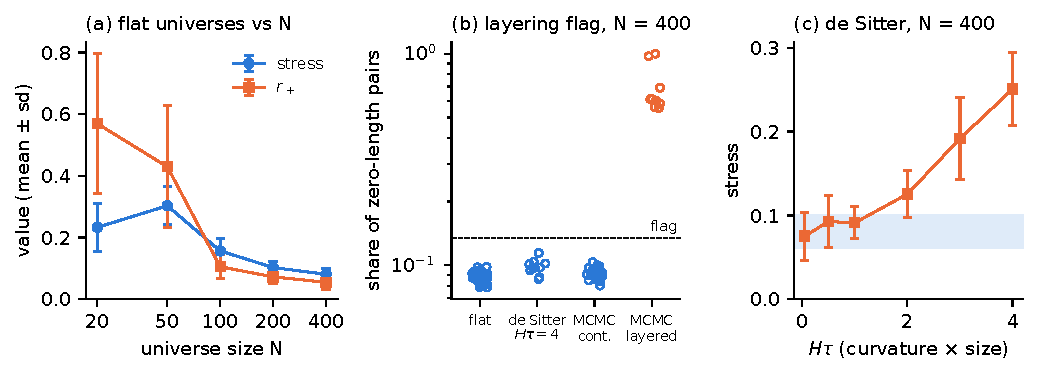
\includegraphics[width=\linewidth]{fig_detector}
\caption{Calibrating the embedding test. (a) Flat universes (random 2D orders, 10 per size, $M=40$): stress and $r_+$ against $N$. (b) Share of zero-length pairs at $N=400$ ($M=80$): flat universes, de Sitter diamonds at $H\tau=4$, and final states of $e^{-\beta S}$ Monte Carlo chains (continuum-like, 30--39 layers; layered, 4--11 layers). Dashed: the flag, $1.5\times$ the flat median. The 13 states with 2--3 layers are not shown. (c) Stress of de Sitter diamonds at fixed $N=400$ (8 per height) against $H\tau$; shaded: the flat band ($\pm1$ sd).}
\label{fig:detector}
\end{figure}

\section{Which 2D orders look like spacetime?}\label{sec:phases}
\paragraph{Classical growth.} In classical sequential growth~\cite{RideoutSorkin00} events are born one at a time and each newborn picks its past among existing events. We grew $N=100$ universes with a fixed link probability $p=0.05$ and with $p_n=3/n$ (an expanding universe from a single first event). Neither gives a $1+1$ spacetime: the ordering-fraction (Myrheim--Meyer) dimension drifts with scale, and the embedding test fails on every number (share of the spectrum in one time and one space direction $\approx0.33$ against $0.65$ for flat universes of the same size, stress $\approx0.65$ against $0.19$). At $N=200$ they still fail on stress ($0.64$--$0.78$ against $\approx0.12$ for flat universes); their zero share is not what flags them. The second rule also uses the birth order as a clock; covariant routes to cosmology in growth models are discussed in~\cite{MORS01,AhmedRideout10}.

\paragraph{The two phases of $e^{-\beta S}$.} Weighting 2D orders by $e^{-\beta S}$, with $S$ the Benincasa--Dowker action, gives a first-order transition between a continuum-like phase and a layered phase~\cite{BHS08,Surya12,GOS18}. We sampled it with Metropolis swap moves at non-locality parameter $\epsilon=0.21$ (an $O(N^2)$ update: a swap changes two rows and columns of the causal matrix). At $N=200$ the test gives:
\begin{center}\small
\begin{tabular}{@{}lccccc@{}}
\toprule
$N=200$ & ordering fraction & layers & $r_+$ & stress & zero share $z$ (fresh chains)\\
\midrule
flat (random orders) & 0.50 & 24 & 0.07 & 0.10 & 0.10--0.15\\
$\beta=0.05$ (continuum-like) & 0.51 & 24 & 0.10 & 0.11 & 0.12--0.13 ($\beta\le0.3$)\\
$\beta=0.6$ (layered) & 0.59 & 9 & 0.39 & 0.28 & 0.39--0.48 ($\beta\ge0.6$, 8--13 layers)\\
\bottomrule
\end{tabular}
\end{center}
(The $\beta\ge0.6$ states are metastable intermediates; the known ground state at large $\beta$ is a bilayer~\cite{CunninghamSurya19}.) We then applied the flag of Sec.~\ref{sec:embed} to 44 final states of $N=400$ chains run from random and from layered starts at $0.01\le\beta\le0.7$. All 22 continuum-like states (30--39 layers) pass; all 9 states with 4--11 layers are flagged ($z=0.55$--$1.0$ against a threshold $0.13$); the 13 states with 2--3 layers break the pipeline. Because the rule was designed after seeing these states, we tested it on fresh $N=200$ chains: 12 of 12 continuum-like states passed and 18 of 18 layered states ($\beta=0.6$--$1.5$) were flagged. These states are test inputs, not equilibrium samples: the chains from layered starts accept $\le0.1\%$ of moves, so we do not use them to locate the transition. Our bracket $0.05<\beta_c(400)<0.45$ is consistent with the finite-size fit $\beta_c\approx1.66/(\epsilon^2N)=0.094$ of~\cite{GOS18}.

\section{A density-free target for Johnston's propagator}\label{sec:prop}
\paragraph{The propagator.} Johnston's particle hops along the order with amplitude $a$ per hop and $b$ per intermediate stop~\cite{Johnston08}. With $C$ the causal matrix ($C_{xy}=1$ if $x\prec y$) and $\Phi=aC$,
\begin{equation}
K=\Phi+b\,\Phi^2+b^2\Phi^3+\dots=\Phi\,(I-b\Phi)^{-1},\qquad a=\tfrac12,\quad b=-m^2/\rho\quad(1+1).
\end{equation}
$K(x,y)$ is a weighted count of chains: $K(x,y)=\tfrac12\sum_k c_k(x,y)\,(-\mu/2)^k$, with $c_k$ the number of $k$-element chains strictly inside $I(x,y)$ and $\mu=m^2/\rho$. In a sprinkled interval of volume $V=\tau^2/2$ the expected number of $k$-chains is $(\rho V)^k/(k!)^2$, so $\langle K\rangle=\tfrac12\sum_k\big(-(m\tau/2)^2\big)^k/(k!)^2=\tfrac12J_0(m\tau)$, the retarded Klein--Gordon propagator~\cite{Johnston08}.

\paragraph{Fixed interval size.} $K$ depends on the order and on $\mu$ only. In a uniformly random 2D order the $n$ events inside an interval form again a uniformly random 2D order, and any $k$ of them form a chain with probability $1/k!$ (the two linear orders must agree on them). So $E[c_k\,|\,n]=\binom nk/k!$~\cite{Pinsky06}, and
\begin{equation}
E[K\,|\,n]=\frac12\sum_{k=0}^n\binom nk\frac{(-\mu/2)^k}{k!}=\frac12L_n\!\Big(\frac\mu2\Big)\;\approx\;\frac12e^{\mu/4}J_0\Big(\sqrt{2\mu(n+\tfrac12)}\Big),
\label{eq:lag}
\end{equation}
a Laguerre polynomial in the interval size. Averaging over Poisson $n$ with mean $\lambda=\rho\tau^2/2$, $\sum_ne^{-\lambda}\frac{\lambda^n}{n!}\binom nk=\frac{\lambda^k}{k!}$, gives back $\tfrac12\sum_k(-\mu\lambda/2)^k/(k!)^2=\tfrac12J_0(m\tau)$: Johnston's result is the Poisson average of Eq.~\eqref{eq:lag}. (A fixed-$n$ chain test exists for maximal chains, whose length distribution in a 2D interval of $n$ elements measures dimension and embeddability~\cite{ABP18}; Eq.~\eqref{eq:lag} sums all chains with the propagator's weights.) The fixed-$n$ form needs no density and no coordinates: every related pair of a causal set supplies its $n$ and its $K$, and Eq.~\eqref{eq:lag} is the target. The identity itself is combinatorics: at $\mu=-2$ and summed over permutations it counts all increasing subsequences, $n!\,L_n(-1)$ (OEIS A002720; ~\cite{LifschitzPittel81}). We did not find its application to the propagator among the 99 papers on arXiv citing~\cite{Johnston08,Johnston09}; later path-sum work averages over sprinklings~\cite{Shuman23,KastratiHinrichsen26}. Expanding in $\mu$, the first term that can fail is the ordering fraction, i.e.\ the Myrheim--Meyer dimension, so the propagator is a resummed tower of dimension tests.

\paragraph{Tests.} Figure~\ref{fig:laguerre} bins all related pairs of an $N=400$ universe by $n$ and compares $\langle K\rangle$ with Eq.~\eqref{eq:lag} at $\mu=0.05$. A random order and continuum-like $e^{-\beta S}$ universes follow the target (rms deviation $0.012$--$0.020$ over all pairs, the same as for random controls, $0.014$--$0.017$). Layered states with $\sim10$ layers deviate with rms $0.07$--$0.10$, five times more, so the propagator also flags the states that the unpatched embedding test missed (Sec.~\ref{sec:embed}). Crystals fail: in a 4-layer order no interval holds more than 9 events, so $K$ never turns negative and the mass never shows; a 7-layer order falls below the target (too many chains). Classically grown universes ($N=1500$) fail systematically, one ($p=0.02$) reaching $|K|\approx10$, far beyond the $1+1$ bound $\tfrac12$.

\paragraph{Curvature at fixed $n$.} In curved $1+1$ spacetime a term $(R\tau^2/48)J_2(m\tau)$ appears~\cite{NXDS17}. In a de Sitter diamond conditioned on $n$ events the order depends only on $(n,H\tau)$, so a fixed-$n$ curvature test exists. We find that the share of related pairs rises by $\approx0.027\,(H\tau)^2$ for $n=10$--$60$, and that the fixed-$n$ propagator is no more sensitive than that share alone (a $3\sigma$ detection at $n=30$, $H\tau=1$ needs 175 intervals either way). The fixed-$n$ propagator thus sees curvature through the known chain-abundance route~\cite{RSS13}; we record this as a negative result.

\begin{figure}[t]
\centering
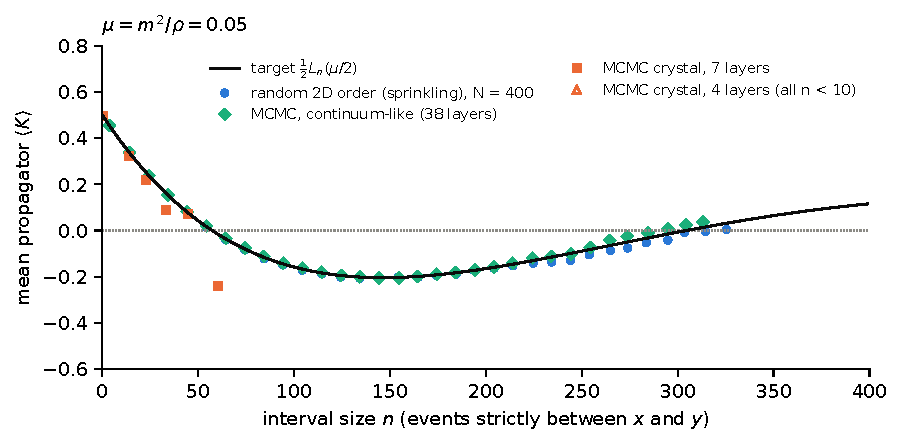
\includegraphics[width=0.92\linewidth]{fig_laguerre}
\caption{Johnston's propagator averaged over related pairs with interval size $n$, against $\tfrac12L_n(\mu/2)$, at $\mu=0.05$ and $N=400$. At large $n$ few pairs remain and the bins are noisy. In the 4-layer crystal every interval has fewer than 10 events, so it contributes a single point near $n=0$.}
\label{fig:laguerre}
\end{figure}

\section{Spatial distances and embedding in $3+1$ dimensions}\label{sec:3p1}
The rectangle identity is special to $1+1$. In $3+1$ dimensions spatial distance from counting is a known open problem~\cite{Surya19}, and the current benchmark is Johnston's embedding~\cite{Johnston25}. This section follows one line. We reproduce his method, locate its error (spacelike pairs whose shared regions hold few events), show that turning those small counts into distances cannot fix it at any size, and then stop turning counts into distances: we fit the coordinates directly to the interval counts of related pairs, each with its Poisson noise, starting from a map built from counts. The likelihood is Casasola's~\cite{Casasola26}; what we add is the intrinsic start and the test against~\cite{Johnston25}. It removes about $80\%$ of his residual error, at every size from $n=3000$ to $15000$ and in every universe. Everything we tried on the way is in App.~\ref{app:dropped}.

\paragraph{Benchmark.} As in~\cite{Johnston25}, $n$ events are sprinkled into a $3+1$ causal diamond of height $1$ (waist radius $\tfrac12$); its bottom and top tips $v_1,v_n$ are added as events. A method returns coordinates from the causal order alone. The score is the Pearson correlation $\rho$ between embedded and true spatial distances over all pairs (his Table~V); we quote the residual $1-\rho$ and, for a new method, the share of his residual it removes, $[(1-\rho_{\rm J})-(1-\rho)]/(1-\rho_{\rm J})$, paired on the same universes. Minkowski correlations (his Table~IV) move the same way and are not shown.

\subsection{Johnston's embedding, reproduced}
Johnston assigns each event a time coordinate from volumes and the proper time of related pairs from interval counts; for a related pair the spatial separation is $R=\sqrt{\Delta t^2-\tau^2}$. For a spacelike pair he takes the shortest detour through an event $z$ related to both,
\begin{equation}
r(x,y)=\min_z\big[R(x,z)+R(z,y)\big],
\end{equation}
an upper bound by the triangle inequality, computed as a min-plus matrix product. Classical MDS on $r$ then gives three spatial coordinates. Our reimplementation reproduces his Table~V, $\rho=0.786$, $0.887$, $0.923$ at $n=500$, $1000$, $1500$ (ten sprinklings each) against his $0.789$, $0.887$, $0.928$, and his Table~III, provided the proper time is computed from the elements strictly between the two events (counting the endpoints, as a literal reading of his definition suggests, gives $0.72$ at $n=1000$; Pellegrin found the same independently~\cite{Pellegrin26}). We did not reproduce his Table~IV ($0.82$, $0.90$, $0.93$ against $0.958$, $0.977$, $0.985$), also not with the true time coordinate, and we suspect a different statistic there; we use the spatial correlation throughout.

\paragraph{Where the error lives.} An oracle test locates it. Replacing his spacelike $r$ by the true spatial distances, and keeping everything else, lifts $\rho$ from $0.903$ to $0.9999$ at $n=1000$ (from $0.915$ to $0.9999$ at $n=1500$). Replacing instead the related-pair values by the truth changes nothing ($0.903\to0.906$). The whole residual of the method is in the spacelike pairs. (Pellegrin, studying the same spacelike fill with link-graph paths, attributes much of the error to noisy related-pair distances on near-collinear pairs~\cite{Pellegrin26}; for Johnston's own two-hop rule our oracle finds that correcting the related pairs does not help.)

\subsection{Distances from small counts}\label{sec:overlap}
\paragraph{An overlap-volume estimator.} Let $a,b$ be spacelike and $c$ an event in their common past. The volumes of $I(c,a)$, $I(c,b)$ and of their overlap $C$ are functions of the proper times $\tau_{ca},\tau_{cb}$ and of the spacelike distance $d$; the first two give $\tau$ through $V=\pi\tau^4/24$. Taking $\tau_{ca}\ge\tau_{cb}$, the overlap measured in units of the smaller interval,
\begin{equation}
w=\frac{V_C}{V_b}=w\Big(\frac{\tau_{cb}}{\tau_{ca}},\frac{d}{\tau_{ca}}\Big)\in[0,1],
\end{equation}
is a function of two ratios only. We tabulate it once by Monte Carlo (common random numbers; $\tau_{cb}/\tau_{ca}\in[0.05,1]$, $d/\tau_{ca}\le8$) and invert it in $d$. On a causal set the volumes are counts; we use $w=(N_C+\tfrac12)/(N_b+1)$, which keeps the inversion finite when $N_C=0$. For the benchmark we take $c=v_1$, so that $d(a,b)$ needs only $|{\rm past}(a)|$, $|{\rm past}(b)|$ and $|{\rm past}(a)\cap{\rm past}(b)|$, and we use the future side ($c=v_n$) instead when it holds more events. Both counts for all pairs come from two matrix products. The same three counts (two pasts and their overlap) also define M\"uller's past-cone metric~\cite{Muller25}, without an inversion to a distance. This is the construction of Bogu\~n\'a and Krioukov~\cite{BK24}: the idea of reading a spacelike distance from the overlap of two causal intervals with a common past event is theirs, and so is the proposal to rebuild space by embedding the resulting distance matrix. They also invert the overlap exactly, numerically and in any dimension, for $c$ at equal proper time below $a$ and $b$ (their Eq.~(22)). What we change is the second argument: we tabulate $w$ for unequal depths, $\tau_{cb}/\tau_{ca}<1$, with both proper times read from counts, so that a single reference event serves all pairs. The Euclidean analogue, distance between two sensors from the counts of their shared and unshared neighbours, is known in sensor-network localization, both as a deterministic inversion~\cite{Buschmann06} and as a maximum-likelihood estimate with a Cram\'er--Rao bound~\cite{Huang14}. On late events of large sprinklings ($N=2\times10^4$--$8\times10^4$) the estimator has a median error of 1--2\% and a bias below 1\% for $d\ge4\ell$, and 6--8\% below $2\ell$.

\paragraph{On the benchmark: good per pair, bad as an embedding.} Table~\ref{tab:profile} splits the spacelike pairs by their true separation. The detour is poor for close pairs, where no $z$ lies between them, and good for far pairs, where many $z$ lie near the straight line; our estimator is the other way round. On the same quantity and the same pairs, our median per-pair error is lower than his ($0.112$ against $0.132$ at $n=1000$, $0.062$ against $0.083$ at $n=3000$; pairs with at least 20 events in the shared region). Yet our estimator alone embeds far worse ($1-\rho=0.18$ against $0.049$ at $n=3000$; Fig.~\ref{fig:3p1}a).

\begin{table}[t]
\centering\small
\begin{tabular}{@{}lrcccc@{}}
\toprule
true $|\Delta x|$ & pairs & ours: bias & ours: error & detour: bias & detour: error\\
\midrule
$0$--$0.1$ & 3\,872 & $-0.05$ & $0.16$ & $+0.40$ & $0.48$\\
$0.1$--$0.2$ & 43\,341 & $-0.16$ & $0.21$ & $-0.08$ & $0.34$\\
$0.2$--$0.35$ & 217\,706 & $-0.17$ & $0.18$ & $-0.12$ & $0.22$\\
$0.35$--$0.5$ & 295\,991 & $-0.14$ & $0.15$ & $-0.07$ & $0.13$\\
$0.5$--$1$ & 230\,652 & $-0.11$ & $0.12$ & $+0.01$ & $0.06$\\
\bottomrule
\end{tabular}
\caption{Spacelike spatial distances by true separation, $n=1500$ (diamond of height 1): median signed bias and median absolute relative error of our estimate (capped by the detour bound) and of Johnston's detour.}
\label{tab:profile}
\end{table}

\paragraph{The low-count pairs are the whole problem.} Let $k$ be the number of events in the shared region on the side used. Pairs with $k<10$ are not a handful: they are $50\%$ of the spacelike pairs at $n=1500$ and $31\%$ at $n=3000$; most of them straddle the waist of the diamond, where both the shared past and the shared future are small. A second oracle replaces our estimate by the truth on the $k<10$ pairs only: this alone removes $88$--$96\%$ of Johnston's residual (3 and 2 universes), while the truth on all the other pairs barely moves our map. Our distances are good wherever $k\ge10$; the embedding fails because classical MDS gives the noisy low-count distances the same voice as the rest.

\paragraph{Why more events do not cure it.} The distance is carried by the events in the past of $b$ that are not in the past of $a$. For small $d$ this region is a shell of thickness $\sim d$ over a cone of height $\tau$, so it holds $\kappa\rho\,d\,\tau^3$ events with $\kappa=O(1)$, and its Poisson fluctuation gives
\begin{equation}
\frac{\delta d}{d}\approx\frac1{\sqrt{\kappa\rho\,d\,\tau^3}}.
\end{equation}
At fixed shape all lengths grow as $n^{1/4}$ in units of $\ell$, so $d\tau^3\propto n$ and $\delta d/d\propto n^{-1/2}$ for the typical pair; the measured median errors fall as $n^{-0.54}$ (ours) and $n^{-0.42}$ (detour) between $n=1000$ and $3000$. The tail is geometric, though: a pair at opposite sides of the waist has a small shared past \emph{and} a small shared future at any $n$. Between $n=6000$ and $15000$ the residual of our estimator alone falls as $\approx n^{-0.4}$, against $\approx n^{-0.85}$ for Johnston (Fig.~\ref{fig:3p1}a). The lesson is not to invert small counts at all.

\subsection{Fitting the coordinates to the counts}\label{sec:likelihood}
\paragraph{Model.} Keep Johnston's time coordinate $t_i$ and treat the $3n$ spatial coordinates $\mathbf x_i$ as unknowns. For a related pair $a\prec b$, the number $N_{ab}$ of events strictly between them is Poisson with mean $\rho\,\pi\tau_{ab}^4/24$, where $\tau_{ab}^2=(t_b-t_a)^2-|\mathbf x_b-\mathbf x_a|^2$. We use this in Gaussian form for $\tau^2$: with $\widehat{\tau^2}_{ab}=\sqrt{(N_{ab}+\tfrac12)/(\rho\pi/24)}$ and $\sigma_{ab}=\widehat{\tau^2}_{ab}/(2\sqrt{N_{ab}+1})$ (a relative error $\delta N/2N$),
\begin{equation}
\ln L(\mathbf x)=-\frac12\sum_{a\prec b}\left(\frac{\tau^2_{ab}(\mathbf x)-\widehat{\tau^2}_{ab}}{\sigma_{ab}}\right)^{\!2},
\label{eq:lik}
\end{equation}
summed over \emph{all} related pairs. The Gaussian form is a convenience, not an approximation that matters: the exact Poisson log-likelihood $\sum[N\ln\mu-\mu]$ gives the same maps (check (v) below), provided it also states that the pair is related; without that, a pair with $N=0$ is fitted best as spacelike, at no cost, and the fit drifts. The Gaussian form, whose target $\widehat{\tau^2}$ is always positive, needs no such term. Spacelike pairs do not enter: each event is pinned by its $O(n)$ related partners, and a pair with many events between it is pinned tightly, one with few loosely, which is exactly the weighting MDS lacked. We maximize Eq.~\eqref{eq:lik} by Adam with the analytic gradient (checked against finite differences), 400 iterations, step $1\%$ of the spatial spread, reduced by $0.3$ halfway; the tips are held at $\mathbf x=0$. Each iteration costs $O(\#\text{related pairs})=O(n^2)$.

\paragraph{Start.} The fit needs a start that is already roughly right, and it must come from the order alone. We use our overlap estimates of Sec.~\ref{sec:overlap}, embedded by weighted stress majorization (SMACOF~\cite{deLeeuwMair09}; accuracy-weighted MDS is standard in sensor localization~\cite{CostaPatwariHero06}) with weight $k/(k+100)$ per spacelike pair and $1$ per related pair, so that low-count distances barely act; this map alone removes $26$--$58\%$ of Johnston's residual (Table~\ref{tab:lik}), fading with $n$. The result of the fit does not depend on this choice: started from Johnston's own map instead, the gain is the same within one percentage point ($74$--$76\%$ at $n=1500$ and $3000$, same universes).

\paragraph{Credit.} Fitting causal-set coordinates to interval counts by a Poisson likelihood is Casasola's~\cite{Casasola26}: a pseudo-likelihood $\sum[N\ln\mu-\mu]$ over related pairs near the light cone ($\tau^2<6\ell^2$) in a $3+1$ diamond, with Langevin draws, started from the \emph{true} positions displaced by about $\ell$, an intrinsic start being left as outlook; it has no comparison with~\cite{Johnston25}. Maximum-likelihood coordinates are standard elsewhere: in multidimensional scaling~\cite{Ramsay77}, latent-space network models~\cite{Hoff02}, hyperbolic maps of the Internet, including a geometric first guess refined by likelihood, as here~\cite{BPK10,Mercator19}, and directed graphs in Minkowski space~\cite{Sim21}. What we add is the intrinsic start, the use of all related pairs, and the test on Johnston's benchmark at large $n$.

\paragraph{Results.} Table~\ref{tab:lik} and Fig.~\ref{fig:3p1}a. The fit beats Johnston's embedding in every one of the 21 universes, and removes a stable $79$--$83\%$ of his residual from $n=3000$ to $15000$ ($67\%$ in the single universe at $n=1000$). Its residual falls as $n^{-0.95}$ against his $n^{-0.85}$ over $n=6000$--$15000$, so the gap is not closing. At $n=15000$ the spatial correlation is $0.9980$ against his $0.9886$. The oracle ceiling of perfect spacelike distances, $0.9999$, is still above it.

\begin{table}[t]
\centering\small
\begin{tabular}{@{}rccccccc@{}}
\toprule
$n$ & univ. & Johnston $\rho$ & likelihood $\rho$ & gain & \multicolumn{3}{c}{share of his $1-\rho$ removed}\\
\cmidrule(l){6-8}
 & & & & & likelihood & weighted start & switch\\
\midrule
3000 & 2 & 0.9515 & 0.9901 & $+0.0386\pm0.0024$ & 80\% & 47\% & 17\%\\
6000 & 4 & 0.9752 & 0.9953 & $+0.0201\pm0.0008$ & 81\% & 38\% & 20\%\\
10000 & 8 & 0.9846 & 0.9968 & $+0.0122\pm0.0003$ & 79\% & 23\% & 19\%\\
15000 & 6 & 0.9886 & 0.9980 & $+0.0094\pm0.0002$ & 83\% & 26\% & 19\%\\
\bottomrule
\end{tabular}
\caption{The likelihood fit, Eq.~\eqref{eq:lik}, against Johnston's embedding on fresh sprinklings, paired on the same universes (cluster runs); errors from the spread of the paired differences (with two universes only indicative). Also shown: the weighted map used as the start, and the hard switch of App.~\ref{app:dropped}.}
\label{tab:lik}
\end{table}

\begin{figure}[t]
\centering
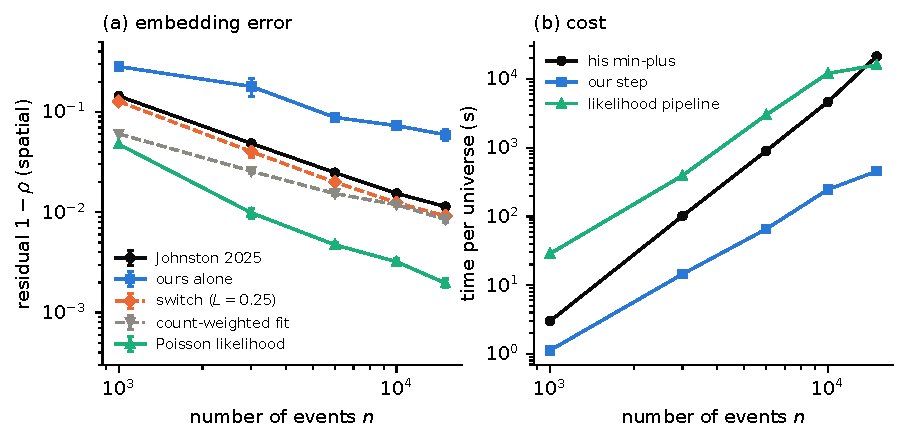
\includegraphics[width=0.95\linewidth]{fig_3p1}
\caption{$3+1$ embedding on Johnston's benchmark, $n=10^3$--$1.5\times10^4$ (1, 2, 4, 8, 6 universes). (a) Residual $1-\rho$ of the spatial correlation for his embedding, our overlap estimator alone, the switch and the weighted map (App.~\ref{app:dropped}), and the likelihood fit. (b) Time per universe on one cluster node shared with other jobs: his min-plus step, our counting step, and the whole likelihood pipeline (counting step, weighted start, 400 iterations).}
\label{fig:3p1}
\end{figure}

\paragraph{Checks.} (i) \emph{Consistency.} Started from the true positions (true times), the fit moves away from the truth only by the finite-$n$ noise and approaches it with $n$: $\rho=0.966$, $0.991$, $0.9965$ at $n=400$, $1000$, $2000$. (ii) \emph{Start independence}: above. (iii) \emph{Ablation.} We also tried adding a term of our own for the spacelike pairs, a binomial likelihood for the Bogu\~n\'a--Krioukov overlap count, $N_C\,|\,N_b\sim{\rm Bin}(N_b,w)$ with $w$ from the table of Sec.~\ref{sec:overlap}. Alone it removes $14$--$25\%$ of his residual; added to Eq.~\eqref{eq:lik} it \emph{lowers} the gain, to $58$--$64\%$ at every $n$. We have not isolated why (the far-pair table bias of Table~\ref{tab:profile}, ratios taken from noisy counts, and pairs treated as independent are candidates). The gain is the related-pair term. (iv) \emph{No tuning on the test universes.} The cluster runs used settings fixed beforehand on other universes; the one hand-set constant, the start's $100$, does not matter by (ii). (v) \emph{Form of the likelihood and convergence.} On the universes of (ii)--(iii) ($n=1500$, 3 universes; $n=3000$, 2), we compared the Gaussian form with the exact Poisson log-likelihood plus a soft relation term $\sum\ln\sigma(\tau^2/s)$, $s=0.1\ell^2$ (cf.\ the soft walls of~\cite{Casasola26}), each at 400 and 1000 iterations. All four remove $76$--$77\%$ ($n=1500$) and $74$--$75\%$ ($n=3000$) of his residual; the paired differences are at most $0.0003$ in $\rho$. Started from the truth, the exact form stays slightly closer ($\rho=0.973$, $0.993$, $0.997$ at $n=400$, $1000$, $2000$). The log-likelihood keeps creeping up after 400 iterations, but the map no longer changes.

\paragraph{A second shape.} A causal diamond has a waist, and Johnston's error is concentrated there. In a slab, a cylinder $t\in[0,1]$, $|\mathbf x|\le\tfrac12$, without tips, he is strong ($\rho=0.985$ at $n=1500$ against $0.926$ in the diamond) and the switch gains nothing. The related-pair likelihood needs no reference event, so it applies unchanged (with no event pinned; we remove the mean of the gradient). To isolate the spatial step, every method here uses the true time coordinate, his detours fall back to four legs when no two-leg detour exists, and our start uses for each pair a reference among 64 events near the lower and upper boundaries. We compare the shapes at equal density: slab $n=6000$ and $12000$ against diamond $n=1500$ and $3000$, 4 universes each (errors are standard errors over universes). The fit removes $58\pm9\%$ and $65\pm6\%$ of his residual in the slab, against $75\pm5\%$ and $80\pm6\%$ in the diamond through the same pipeline. The difference is at the side wall. A diamond contains every interval between its events (it is order-convex); a slab is not, and, as Pellegrin noted for slab-shaped cuts of a diamond~\cite{Pellegrin26}, an interval that pokes out of the wall has too few events, so its pair looks closer to null than it is: $45\%$ of related pairs lose some of their interval and $14\%$ lose more than a fifth, at every $n$. Dividing each count by the true share of its interval inside the slab (an oracle, for diagnosis only) raises the slab result to $80\%$ and $86\%$, level with the diamond: at equal density the wall accounts for the whole gap. Its cost, about $20$ percentage points, does not shrink with $n$, because the share of clipped intervals is set by the shape. On interior pairs (both events in the top quartile of $\min(|{\rm past}|,|{\rm future}|)$) the slab does at least as well as the diamond ($80\pm12\%$ and $86\pm2\%$, against $69\pm10\%$ and $71\pm14\%$). We do not correct for the wall, since a correction needs the shape of the region. Two caveats. These shares are of a small residual: in the slab his $1-\rho$ is $0.0069$ and $0.0047$, about ten times below the diamond's. And the gain needs density: in the slab it falls to $43\pm10\%$ at $n=1500$ (3 universes), and in a single slab universe at $n=600$ the fit does worse than his embedding.

\subsection{Cost}
Fig.~\ref{fig:3p1}b gives the time per universe on one cluster node (4 cores, shared with other jobs, so exponents are rough). His min-plus step grows as $\approx n^{3}$--$n^{3.5}$; our counting step, two dense matrix products and a table look-up, as $\approx n^{2}$; the likelihood pipeline costs $O(n^2)$ per iteration at a fixed 400 iterations. At $n=3000$--$6000$ the pipeline is $3$--$4$ times slower than his min-plus step, at $n=10^4$ about $2.5$ times, and at $n=15000$ somewhat faster ($1.6\times10^4$ against $2.1\times10^4$\,s, mean over 6 universes on loaded nodes). The fit's time at $n=15000$ equals its time at $10^4$, which a fixed number of $O(n^2)$ iterations does not explain; we have not resolved this, and it may be node load. The claim is accuracy, not speed. At 400 iterations the log-likelihood still creeps up ($0.01$--$0.05\%$ per 100 iterations in the cluster runs), but 1000 iterations give the same maps at $n\le3000$ (check (v)); whether that holds at much larger $n$ is open.

\subsection{Limitations of the $3+1$ result}
The tables are flat-space tables and the likelihood assumes a flat interval volume; in curved spacetime the volumes carry corrections of order $R\tau^2$ (the depth drift of Sec.~\ref{sec:curv} is the $1+1$ case), which would bias the fit in a way that grows with depth. The time coordinate is Johnston's and is not refitted. The benchmark is a flat diamond; in the second shape the side wall costs about $20$ percentage points at every size, and the gain needs density (it is lost in one slab universe at $n=600$).

\section{Discussion}\label{sec:disc}
\paragraph{What is new, and what we checked.} The overlap regions are from~\cite{BK24} and the embedding from~\cite{CloughEvans16}; the zero-share flag is a relative of~\cite{GlaserSurya13}, and the Laguerre identity is classical combinatorics. To our knowledge the following are new: the general-$c$ rectangle identity, Eq.~\eqref{eq:rect}, with the bias-corrected estimator; the depth-drift curvature estimator and its closed form, Eq.~\eqref{eq:drift}; the calibration of the embedding test against size, curvature and layering; and the fixed-$n$ target, Eq.~\eqref{eq:lag}. For each we read the full citation lists of the closest papers (\cite{BK24}, \cite{CloughEvans16}, \cite{Johnston08,Johnston09}) and searched the full texts; the rectangle identity is elementary enough that it may appear in passing somewhere we did not look. In $3+1$ the overlap regions are again from~\cite{BK24}, the time coordinate is Johnston's~\cite{Johnston25}, and the likelihood of related-pair counts is Casasola's~\cite{Casasola26}; maximum-likelihood coordinates are standard in other fields~\cite{Ramsay77,Hoff02,BPK10,Mercator19,Sim21}. What we add is the tabulated overlap inversion for unequal depths (Bogu\~n\'a and Krioukov invert it exactly for equal depths, their Eq.~(22), and on a causal set keep only reference events at equal depth, their Eqs.~(32)--(34)~\cite{BK24}; the full texts of their seven INSPIRE citers and of~\cite{RideoutWallden09} contain no unequal-depth version), the reproduction and oracle analysis of~\cite{Johnston25} with the low-count diagnosis, the counting argument for why inverted distances cannot close the gap, the intrinsic start, and the large-$n$ test, ablation and second shape. Casasola's and Pellegrin's preprints are not on arXiv or INSPIRE. Beyond arXiv and INSPIRE we searched OpenAlex, Crossref, Zenodo, GitHub, Research Square and SSRN (through OpenAlex and Crossref), theses and the general web (about 200 queries and 60 full texts, October 2026); Google Scholar, thesis full-text databases and conference abstract books were not searched systematically, and similar work outside the databases we reached may exist. At the time of writing~\cite{Johnston25} has one citing paper on INSPIRE, which reconstructs curvature from counts with local charts rather than distances~\cite{Madsen26}.

\paragraph{Limitations.} The exact results are $1+1$. The rectangle identity has no direct analogue in higher dimensions, where the overlap of two intervals is not an interval. Our $3+1$ results are numerical: mainly one benchmark (a flat causal diamond), with 2--8 universes per size at large $n$, Johnston's time coordinate kept fixed, flat-space volumes, and 400 iterations (enough at $n\le3000$); the second shape is tested at one size so far (Sec.~\ref{sec:likelihood}). The curvature estimator is noisy (about 100 pairs for $\pm20\%$) and was tested on de Sitter and one FRW spacetime; it measures a depth-weighted average of $R$. The embedding thresholds are empirical and must be recalibrated at each $N$; the $e^{-\beta S}$ states we used are test inputs, not equilibrium samples. The Laguerre target is exact only for 2D orders.

\paragraph{Outlook.} In $3+1$ the oracle still leaves room ($\rho=0.9999$ against $0.998$ at $n=15000$). Natural next steps are to refit the time coordinate together with space, to model the boundary of regions that are not causally convex, and to replace the flat interval volume by a curved one, perhaps with the normal-coordinate construction of~\cite{Madsen26}, which would turn the fit into a curvature estimator as in $1+1$. Beyond distances, two extensions look natural: a version of the depth drift built from Hu--Meyer--Meyer's past-and-future construction~\cite{HMM25}, which may be less noisy, and a fixed-$n$ target in $3+1$. There the exactness of Eq.~\eqref{eq:lag} is lost: Johnston's $3+1$ particle hops along links only~\cite{Johnston08}, so a path requires every skipped sub-interval to be empty, and $E[K\,|\,n]$ becomes a sum of $(k-1)$-point integrals with factors $(1-W/V)^{n-k+1}$. Its first term can be done for large $n$: the expected number of two-hop link paths tends to $3\pi$, which is what Johnston's amplitudes require to reproduce the short-distance limit $m^2/8\pi$ of the continuum mass term~\cite{Johnston08}, so this is a consistency check rather than a new result; a Monte Carlo check approaches it as $3\pi(1-1.6/\sqrt n)$ at fixed $n$. A $3+1$ target is therefore a computed table rather than a formula.

\section*{Code and data}
\sloppy
All simulations are short numpy scripts; the figures are produced by \texttt{sims/fig\_part1.py}, the detector fix by \texttt{sims/r8\_detector\_spread.py}, the curvature fit and the FRW check by \texttt{sims/r9\_drift\_fit\_frw.py}, and the $N=400$ Monte Carlo states by \texttt{sims/n400\_crystal.py}. In $3+1$: the overlap table and estimator in \texttt{sims/r11\_4d\_distance.py}, the reproduction of~\cite{Johnston25} and the oracle in \texttt{sims/r12\_johnston\_compare.py}, the low-count diagnosis in \texttt{sims/r18\_waist\_oracle.py}, the weighted start in \texttt{sims/r19\_cluster\_wfit.py}, the likelihood in \texttt{sims/r23\_likelihood.py} and its cluster runs in \texttt{sims/r24\_cluster\_lik.py}, the second shape in \texttt{sims/r22\_slab.py} and \texttt{sims/r25\_slab\_lik.py}, the switch in \texttt{sims/r13\_mixed.py} and \texttt{sims/r14\_cluster\_scale.py}, and Fig.~\ref{fig:3p1} by \texttt{sims/fig\_3p1.py}. Repository, with the full research notebook: \url{https://github.com/presindev/causet-counting}.

\section*{Acknowledgements, funding and use of AI tools}
% arXiv policy: AI tools cannot be authors; their use must be disclosed (wording approved by Roberto, session 14).
This work was funded by SapereIA. Simulations were run on the Nyx cluster of the Institute of Cosmos Sciences of the University of Barcelona (ICCUB). An AI system (Claude Opus~5.5, Anthropic) was used throughout, as described in Sec.~\ref{sec:method}; it is not an author. The author takes full responsibility for the content.

\appendix
\section{Paths dropped}\label{app:dropped}
In $3+1$, before the likelihood fit, we tried to make inverted distances win, alone or combined with Johnston's detours. Each item was tested on the same universes as the method it is compared with.
\begin{itemize}[leftmargin=*,itemsep=1pt]
\item \emph{A hard switch} (the author's suggestion): our estimate if it says the pair is closer than $L=0.25$, his detour otherwise. Held out at $n=500$--$3000$ ($L$ chosen on other universes) and on the cluster up to $n=15000$, it beat him in every universe, removing a stable $17$--$20\%$ of his residual (Table~\ref{tab:lik}); it was our main $3+1$ result until the likelihood fit. In the slab it gains nothing: its gain lives at the waist.
\item \emph{A count-weighted map} (SMACOF, weight $k/(k+K_0)$ per spacelike pair): $42$--$45\%$ of his residual at $n\le3000$, but the share fades with $n$ (to $23$--$36\%$ at $n=10^4$--$1.5\times10^4$ for $K_0=100$--$300$) and depends on the hand-set $K_0$. Kept only as the start of the fit.
\item \emph{A binomial likelihood term} for the overlap counts of spacelike pairs, our construction: lowers the fit's gain by $15$--$20$ points at every $n$ (Sec.~\ref{sec:likelihood}).
\item \emph{A map from counts only} (SMACOF with far pairs at weight $0.1$, no detours): matched him up to $n=3000$, lost at larger $n$ ($-14\%$ to $-31\%$ of his residual).
\item \emph{Laplacian eigenmaps}, suggested in~\cite{BK24}: capped at $\rho\approx0.93$ even on the true distances, because the eigenfunctions of a ball are not linear coordinates.
\item \emph{Local trilateration charts} after~\cite{Madsen26}: exact on true intervals, but $30$--$42\%$ per-pair error from counts at $n\le3000$ (ill-conditioned Gram matrices).
\item \emph{Johnston's detour on the low-count pairs only}: no better than his embedding; his detours are no better there than ours.
\item \emph{Averaging} our estimate with his detour: worse than his alone ($-0.07$ to $-0.006$).
\item \emph{Several reference events} instead of $v_1$, averaged: no gain; deep references see the same region.
\item \emph{Both sides} (past and future references) combined with Poisson weights: worse than taking the side with more events.
\item \emph{Our estimate capped by his upper bound}: better than ours alone, but its residual stays $\approx2.5$ times his.
\item \emph{Chained detours}, routes through his related edges and our short estimates: much worse ($-0.06$ to $-0.29$). Our short legs are biased low and the minimum over many routes picks the lowest, so the bias compounds.
\item \emph{Random stepping stones} for a cheaper detour: at or below him ($-0.008$ to $-0.033$ at $n=3000$); a far pair needs a stone related to both events, and random events rarely are.
\item \emph{Chosen stepping stones} near the midpoint of each far pair, located on a rough first map: keeps about two thirds of the switch's gain at $n=3000$ (one third at $1500$) at a quarter of the far-pair time, but the cost is still cubic at fixed grid size.
\item In the counts-only map, \emph{dropping} the far pairs instead of down-weighting them: $-0.012$ at $n=3000$.
\end{itemize}

\begin{thebibliography}{99}\small
\bibitem{BLMS87} L.~Bombelli, J.~Lee, D.~Meyer, R.~D.~Sorkin, ``Space-time as a causal set'', Phys.\ Rev.\ Lett.\ 59, 521 (1987).
\bibitem{Surya19} S.~Surya, ``The causal set approach to quantum gravity'', Living Rev.\ Rel.\ 22, 5 (2019), arXiv:1903.11544.
\bibitem{BrightwellGregory91} G.~Brightwell, R.~Gregory, ``Structure of random discrete spacetime'', Phys.\ Rev.\ Lett.\ 66, 260 (1991).
\bibitem{RSS13} M.~Roy, D.~Sinha, S.~Surya, ``The discrete geometry of a small causal diamond'', Phys.\ Rev.\ D 87, 044046 (2013), arXiv:1212.0631.
\bibitem{GlaserSurya13} L.~Glaser, S.~Surya, ``Towards a definition of locality in a manifoldlike causal set'', Phys.\ Rev.\ D 88, 124026 (2013), arXiv:1309.3403.
\bibitem{BD10} D.~M.~T.~Benincasa, F.~Dowker, ``The scalar curvature of a causal set'', Phys.\ Rev.\ Lett.\ 104, 181301 (2010), arXiv:1001.2725.
\bibitem{DowkerGlaser13} F.~Dowker, L.~Glaser, ``Causal set d'Alembertians for various dimensions'', Class.\ Quant.\ Grav.\ 30, 195016 (2013), arXiv:1305.2588.
\bibitem{BK24} M.~Bogu\~n\'a, D.~Krioukov, ``Measuring spatial distances in causal sets via causal overlaps'', Phys.\ Rev.\ D 110, 024008 (2024), arXiv:2401.17376.
\bibitem{HMM25} C.~A.~Hu, D.~A.~Meyer, E.~J.~Q.~Meyer, ``Reconstructing Minkowski geometry from causal separations'', J.\ Math.\ Phys.\ 66, 122502 (2025), arXiv:2601.03280.
\bibitem{CloughEvans16} J.~R.~Clough, T.~S.~Evans, ``Embedding graphs in Lorentzian spacetime'', PLoS ONE 12, e0187301 (2017), arXiv:1602.03103.
\bibitem{Henson06} J.~Henson, ``Constructing an interval of Minkowski space from a causal set'', Class.\ Quant.\ Grav.\ 23, L29 (2006), gr-qc/0601069.
\bibitem{Johnston25} S.~Johnston, ``Simpler embeddings of causal sets into Minkowski spacetime'', Phys.\ Rev.\ D 111, 106020 (2025), arXiv:2502.09701.
\bibitem{Johnston08} S.~Johnston, ``Particle propagators on discrete spacetime'', Class.\ Quant.\ Grav.\ 25, 202001 (2008), arXiv:0806.3083.
\bibitem{Johnston09} S.~Johnston, ``Feynman propagator for a free scalar field on a causal set'', Phys.\ Rev.\ Lett.\ 103, 180401 (2009), arXiv:0909.0944.
\bibitem{BHS08} G.~Brightwell, J.~Henson, S.~Surya, ``A 2D model of causal set quantum gravity: the emergence of the continuum'', Class.\ Quant.\ Grav.\ 25, 105025 (2008), arXiv:0706.0375.
\bibitem{Surya12} S.~Surya, ``Evidence for the continuum in 2D causal set quantum gravity'', Class.\ Quant.\ Grav.\ 29, 132001 (2012), arXiv:1110.6244.
\bibitem{BDJ99} J.~Baik, P.~Deift, K.~Johansson, ``On the distribution of the length of the longest increasing subsequence of random permutations'', J.\ Amer.\ Math.\ Soc.\ 12, 1119 (1999).
\bibitem{BBR26} J.~Barton, S.~Borza, J.~R\"ohrig, ``Ollivier--Ricci curvature for causal sets'', arXiv:2606.04910 (2026).
\bibitem{RideoutSorkin00} D.~P.~Rideout, R.~D.~Sorkin, ``Classical sequential growth dynamics for causal sets'', Phys.\ Rev.\ D 61, 024002 (2000).
\bibitem{MORS01} X.~Mart\'in, D.~O'Connor, D.~P.~Rideout, R.~D.~Sorkin, ``On the renormalization transformations induced by cycles of expansion and contraction in causal set cosmology'', Phys.\ Rev.\ D 63, 084026 (2001).
\bibitem{AhmedRideout10} M.~Ahmed, D.~Rideout, ``Indications of de Sitter spacetime from classical sequential growth dynamics of causal sets'', Phys.\ Rev.\ D 81, 083528 (2010).
\bibitem{GOS18} L.~Glaser, D.~O'Connor, S.~Surya, ``Finite size scaling in 2d causal set quantum gravity'', Class.\ Quant.\ Grav.\ 35, 045006 (2018), arXiv:1706.06432.
\bibitem{CunninghamSurya19} W.~J.~Cunningham, S.~Surya, ``Dimensionally restricted causal set quantum gravity: examples in two and three dimensions'', Class.\ Quant.\ Grav.\ 37, 054002 (2020), arXiv:1908.11647.
\bibitem{Pinsky06} R.~G.~Pinsky, ``Law of large numbers for increasing subsequences of random permutations'', Random Struct.\ Alg.\ 29, 277 (2006), arXiv:math/0407353, eq.~(1.1).
\bibitem{LifschitzPittel81} V.~Lifschitz, B.~Pittel, ``The number of increasing subsequences of the random permutation'', J.\ Combin.\ Theory A 31, 1 (1981) (not read by us; cited via OEIS A002720).
\bibitem{Shuman23} S.~Shuman, ``Path sums for propagators in causal sets'', Phys.\ Rev.\ D 109, 046008 (2024), arXiv:2307.08864.
\bibitem{KastratiHinrichsen26} A.~Kastrati, H.~Hinrichsen, ``Numerical evaluation of the causal set propagator in 2D anti-de Sitter spacetime'', Phys.\ Rev.\ D 113, 065003 (2026), arXiv:2504.12919.
\bibitem{NXDS17} Nomaan~X, F.~Dowker, S.~Surya, ``Scalar field Green functions on causal sets'', Class.\ Quant.\ Grav.\ 34, 124002 (2017), arXiv:1701.07212.
\bibitem{deLeeuwMair09} J.~de~Leeuw, P.~Mair, ``Multidimensional scaling using majorization: SMACOF in R'', J.\ Stat.\ Softw.\ 31(3), 1 (2009).
\bibitem{Casasola26} G.~Casasola, ``Causal sets that locate and grow themselves: sub-discreteness self-localization and order-intrinsic sequential growth of 3+1 Minkowski orders'', Research Square preprint (5 October 2026), doi:10.21203/rs.3.rs-11223018/v1.
\bibitem{Ramsay77} J.~O.~Ramsay, ``Maximum likelihood estimation in multidimensional scaling'', Psychometrika 42, 241 (1977).
\bibitem{Hoff02} P.~D.~Hoff, A.~E.~Raftery, M.~S.~Handcock, ``Latent space approaches to social network analysis'', J.\ Amer.\ Statist.\ Assoc.\ 97, 1090 (2002).
\bibitem{BPK10} M.~Bogu\~n\'a, F.~Papadopoulos, D.~Krioukov, ``Sustaining the Internet with hyperbolic mapping'', Nat.\ Commun.\ 1, 62 (2010), arXiv:1009.0267.
\bibitem{Mercator19} G.~Garc\'ia-P\'erez, A.~Allard, M.~\'A.~Serrano, M.~Bogu\~n\'a, ``Mercator: uncovering faithful hyperbolic embeddings of complex networks'', New J.\ Phys.\ 21, 123033 (2019), arXiv:1904.10814.
\bibitem{Sim21} A.~Sim, M.~Wiatrak, A.~Brayne, P.~Creed, S.~Paliwal, ``Directed graph embeddings in pseudo-Riemannian manifolds'', ICML 2021, arXiv:2106.08678.
\bibitem{Buschmann06} C.~Buschmann, D.~Pfisterer, S.~Fischer, ``Estimating distances using neighborhood intersection'', IEEE Conf.\ Emerging Technologies and Factory Automation (ETFA) 2006.
\bibitem{Huang14} B.~Huang, C.~Yu, B.~D.~O.~Anderson, G.~Mao, ``Estimating distances via connectivity in wireless sensor networks'', Wirel.\ Commun.\ Mob.\ Comput.\ 14, 541 (2014), doi:10.1002/wcm.2204.
\bibitem{CostaPatwariHero06} J.~A.~Costa, N.~Patwari, A.~O.~Hero, ``Distributed weighted-multidimensional scaling for node localization in sensor networks'', ACM Trans.\ Sensor Networks 2, 39 (2006).
\bibitem{EMLW26} A.~Eichhorn, H.~Mack, K.~T.~Le, F.~Wagner, ``Charting causal set configuration space with graph observables'', arXiv:2605.27514 (2026).
\bibitem{RideoutWallden09} D.~Rideout, P.~Wallden, ``Spacelike distance from discrete causal order'', Class.\ Quant.\ Grav.\ 26, 155013 (2009), arXiv:0810.1768.
\bibitem{Clough17} J.~R.~Clough, ``Causal structure in networks'', PhD thesis, Imperial College London (2017), hdl:10044/1/50162.
\bibitem{ABP18} M.~E.~Aghili, L.~Bombelli, B.~B.~Pilgrim, ``Path length distribution in two-dimensional causal sets'', Eur.\ Phys.\ J.\ C 78, 744 (2018), arXiv:1805.07312.
\bibitem{Pellegrin26} G.~Pellegrin, ``Link-restricted path filling for causal set embeddings'', Zenodo preprint (5 August 2026), doi:10.5281/zenodo.21813653.
\bibitem{Muller25} O.~M\"uller, ``On the Hauptvermutung of causal set theory'', arXiv:2503.01719 (2025).
\bibitem{Madsen26} N.~Madsen, ``Reconstruction of the Riemann tensor from causal order and element counts'', arXiv:2610.36695 (2026).
\end{thebibliography}
\end{document}
